\section{Results Individual Differences}

This section addresses the secondary research question that involved an investigation of possible individual differences in brain activation related to sensitivity, and if the use of FSL FIX would in increase any findings. The amount positive and negative brain activation related to the pain sensitivity of each individual in the test population can be seen in \figref{STD_pos_ID} and \figref{STD_neg_ID} when preprocessing the data using standard preprocessing.  

\begin{figure}[H]                 
	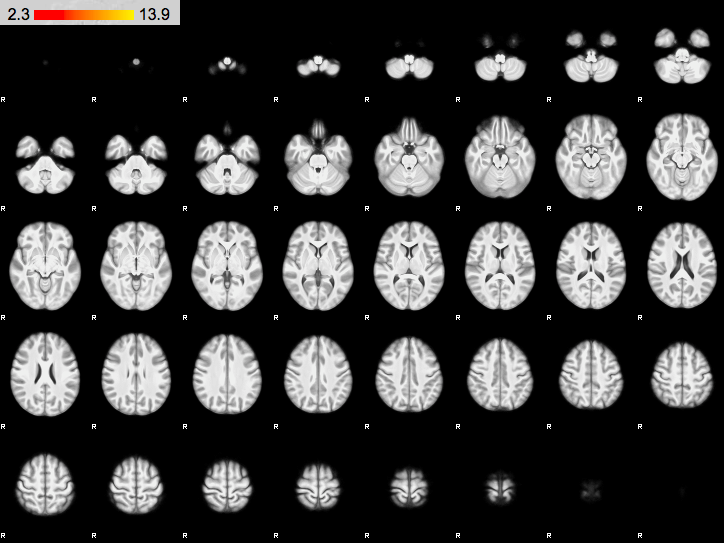
\includegraphics[width=.65\textwidth]{figures/Results/STD_pos_ID}  
	\caption{Positive activation map showing any possible brain regions related to the individual perception of pain after the use of standard preprocessing. }
	\label{STD_pos_ID} 
\end{figure}

\begin{figure}[H]                 
	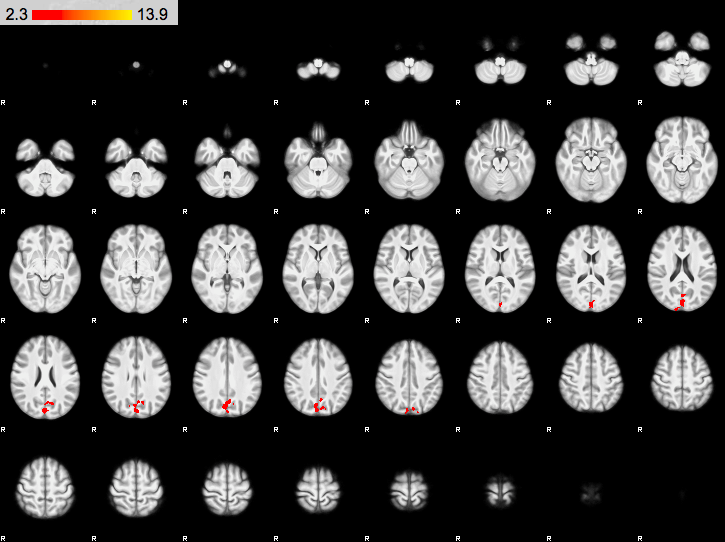
\includegraphics[width=.65\textwidth]{figures/Results/STD_neg_ID}  
	\caption{Negative activation map showing any possible brain regions related to the individual perception of pain after the use of standard preprocessing.}
	\label{STD_neg_ID} 
\end{figure}
 
It is seen that neither positive or negative activation is present in any areas of the brain. Only a very small activation is seen in the negative activation map, but as it is localized between brain hemispheres it is most likely of artifactual nature. The amount of general brain activation presented in \secref{sec:comp}, found by using standard preprocessing does not seem to bring out the activation that might be related to individual differences, if the presence of these would be the case. \\
Using FSL FIX for preprocessing resulted in a higher signal-to-noise ratio, but even when achieving this, it had no impact on the discovery of any possible individual differences. This can be seen on \figref{FIX_pos_ID} and \figref{FIX_neg_ID}, were no activation is seen on the positive or negative map, respectively. The only difference of using FSL FIX it the negative activation found using standard preprocessing is now removed, increasing the likelihood of being noise related. 

\begin{figure}[H]                 
	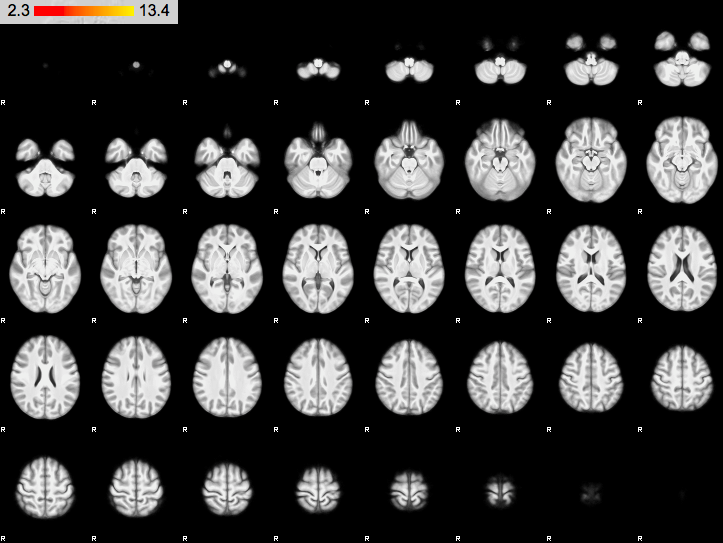
\includegraphics[width=.65\textwidth]{figures/Results/FIX_pos_ID}  
	\caption{Positive activation map showing any possible brain regions related to the individual perception of pain after the use of FIX for preprocessing.}
	\label{FIX_pos_ID} 
\end{figure}

\begin{figure}[H]                 
	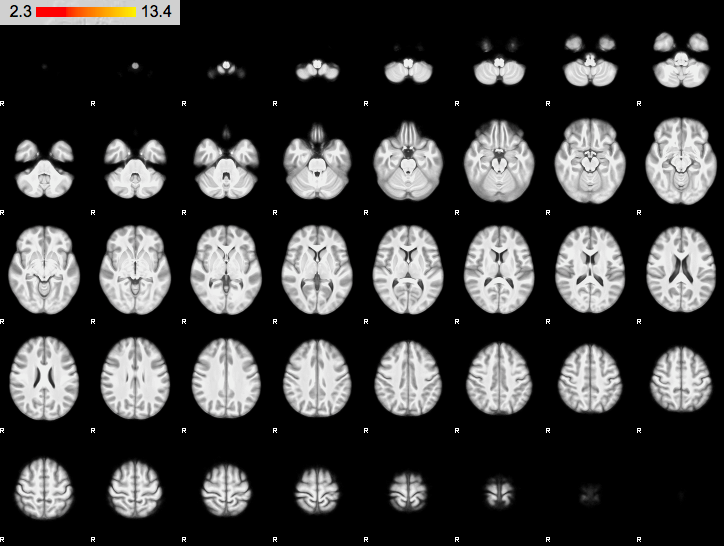
\includegraphics[width=.65\textwidth]{figures/Results/FIX_neg_ID}  
	\caption{Negative activation map showing any possible brain regions related to the individual perception of pain after the use of FIX for preprocessing.}
	\label{FIX_neg_ID} 
\end{figure}


















%Achieving an optimal signal to noise ratio when preprocessing task related fMRI is very desirable. The BOLD signal can be corrupted by physiological noise of non interest, subject movement and scanner artifacts. In addition, higher tesla scanners introduce the risk of more noise. A often applied method for finding noise sources is to use ICA, where the signal is broken down to components of signal and noise, which facilitates the possibility of removing those of non interest. This approach can be very time consuming on larger datasets, pushing the need for automatic noise removal algorithms.
%The aim of the project was to investigate if using the automatic de-noising tool FSL FIX would provide a greater signal to noise ratio compared to a pipeline of standard preprocessing in relation to an investigation of individual differences to a noxious heat stimuli.      